\documentclass[conference]{IEEEtran}
\usepackage{amsmath,amssymb,graphicx,booktabs,url}
\usepackage[hidelinks]{hyperref}
\hypersetup{pdftitle={Conservative Coast-Wide Localization from Unassociated Global Bearings to Charted Aids},pdfauthor={J.C. Vaught}}
\newcommand{\angdist}{\operatorname{dist}_{\mathbb S^1}}
\newcommand{\wrap}{\operatorname{wrap}}
\title{Conservative Coast-Wide Localization from\\Unassociated Global Bearings to Charted Aids}
\author{\IEEEauthorblockN{J.C. Vaught}}
\begin{document}
\maketitle
\begin{abstract}
Bearing-only localization against a coastal chart requires simultaneous position search and association of observations with physical navigation aids. This paper presents a deterministic hierarchical method that covers a declared coastal domain while rejecting only regions with a supported impossibility proof. A true-north bearing enclosure accounts for observer-cell extent, chart-position uncertainty, and numerical margins. A bipartite graph tests whether every trusted aid report can receive a distinct possible chart object. Missing aids incur no penalty, and vessel detections create no chart-aid obligation. Spatial indexes, reusable prepared geometry, device-resident subdivision, parallel visibility prediction, and cooperative assignment concentrate computation on surviving regions. A recorded Eastern Seaboard search for one corrected simulated Charleston frame evaluated 64,875 regions from 39,435 initial cells in 8.462 s on three graphics processing units. The selected terminal center matched all 64 aid reports and lay 2.060 m from independently evaluated truth. The traversal retained 397 terminal cells, including 182 unresolved centers near the selected estimate. These results demonstrate rapid complete-domain traversal for this frame while distinguishing whole-cell exclusion, pointwise consistency, and unresolved local ambiguity.
\end{abstract}
\begin{IEEEkeywords}
Bearing-only localization, chart aids, bounded error, data association, conservative pruning, parallel search.
\end{IEEEkeywords}

\section{Introduction}
A coastal observer can measure directions to navigation aids without measuring their ranges or recognizing their individual chart identities. When its heading is known relative to true north, each direction constrains position directly in a global angular frame. However, a large chart contains many alternative landmark arrangements. A plausible local angular fit therefore does not establish that the observer is in the correct harbor. The search must account for the complete declared domain while treating unavailable detections and incomplete visibility conservatively.

This problem combines geometric resection with combinatorial association. Bearings to identified landmarks already support robot localization \cite{Betke1997LandmarkLocalization}, but chart objects must first be assigned to the observed directions here. Independent nearest-angle assignments can reuse one aid for multiple detections and create a false explanation. Meanwhile, rejecting a location because an expected aid was not detected would impose an additional detection-completeness assumption. The method instead treats observed aids as positive obligations and permits unobserved catalog objects.

The central computational choice is to test regions before scoring positions. Large rectangles are discarded when no position inside can explain the positive measurements. Surviving rectangles are subdivided, causing geometric uncertainty to contract and enabling stronger proofs at finer scales. Expensive shoreline prediction and exact nominal assignment are then concentrated on the small terminal population. Thus, the coast-wide domain is covered by a hierarchy of region decisions rather than by an exhaustive fine grid.

This paper explains the resulting bounded-error model, safe region tests, distinct-object association, and parallel execution strategy. It then analyzes the existing corrected Charleston record \cite{Vaught2026CharlestonRecord}. The evaluation uses archived search outputs, timing records, and an independently frozen estimate.

\section{Related Geometric and Association Methods}
Bearing resection and set-membership estimation supply complementary precedents. Betke and Gurvits estimate position and orientation using bearings to landmarks with known identities \cite{Betke1997LandmarkLocalization}. Colle and Galerne formulate multiangulation through bounded-error set inversion \cite{Colle2013SetInversion}. The present formulation adopts a feasible-set interpretation but includes unknown correspondence, chart completeness, and land occlusion. Known global heading removes orientation from the search state and leaves a two-dimensional position domain.

Association must also be tested jointly. Neira and Tard\'os show that individually compatible matches need not form a jointly compatible assignment in stochastic mapping \cite{Neira2001JointCompatibility}. Here, compatibility is deterministic and interval-based rather than covariance-based. Its central combinatorial condition is injectivity. Hall's representative theorem characterizes when every report can receive a distinct neighboring object \cite{Hall1935Representatives}. Maximum bipartite matching tests this requirement without enumerating all permutations.

Global geometric search also benefits from bounds over regions. Go-ICP combines branch-and-bound with geometric error bounds for globally optimal rigid point-set registration \cite{Yang2016GlobalRegistration}. The present search uses subdivision and impossibility bounds, but does not use an incumbent residual to discard all inferior regions or certify a continuous global residual optimum. It retains every region not disproved at the stopping scale. This distinction separates exhaustive domain coverage from optimality of the selected sampled center.

Finally, the coastal scale requires a consistent geographic frame. Ellipsoidal inverse geodesics provide distance and forward azimuth between observer and chart objects, with differential quantities that support sensitivity reasoning \cite{Karney2013Geodesics}. The angular enclosure below is a derived bound used by this method. It is not an uncertainty guarantee stated by that reference for the particular numerical implementation.

\section{Observation and Map Model}
\subsection{Positive Measurements and Known Heading}
Let $\mathbf{x}$ denote observer position in a declared two-dimensional domain $\mathcal D$, and let $\mathbf{q}_j$ denote chart-object positions. The sensor observes the full $360^\circ$ azimuth range. True-north heading is supplied, so each measured bearing $z_i$ is global rather than relative to unknown vessel yaw. The forward model uses the WGS84 ellipsoidal initial azimuth $\beta(\mathbf{x},\mathbf{q}_j)$. Circular distance is
\begin{equation}
 \angdist(\alpha,\gamma)=|\wrap(\alpha-\gamma)|,
 \label{eq:circular}
\end{equation}
where $\wrap$ returns an angle in $[-\pi,\pi)$. Angular wraparound therefore introduces no special gap between measurements near north.

Let $\mathcal I$ contain trusted physical-aid reports from one simultaneous view. Each report represents a real aid detection. Different reports require distinct physical explanations, while individual aid identities are unknown. Extra detections are vessels only, and known vessel reports are excluded from the aid obligations. The recorded aid-only estimator does not use a vessel-traffic likelihood or require that every catalog object be detected.

For an assignment $\pi$ from reports to physical chart objects, the ideal positive constraint is
\begin{equation}
 \angdist\!\left(z_i,\beta(\mathbf{x},\mathbf{q}_{\pi(i)})\right)
 \leq \tau_i,\qquad i\in\mathcal I,
 \label{eq:point}
\end{equation}
with $\pi$ injective and selected objects visible and within sensor range. The hard sensor tolerance is $\tau_i=0.5^\circ$ for the recorded frame. Known object extents, position support, and numerical margins enter the conservative region model separately.

The corrected simulator draws Gaussian-shaped angular error by rejection sampling within $\pm0.5^\circ$, using an underlying standard deviation of $1/6^\circ$. Rejection sampling preserves a truncated Gaussian shape rather than accumulating probability at clipped endpoints. The hard bound supplies the exclusion tolerance. The distribution's standard deviation does not supply a deterministic bound. This frame uses no deliberate bearing outliers or type errors, a detection probability of $0.9$, and vessel-only extra reports \cite{Vaught2026CharlestonRecord}.

\subsection{Physical Identity and Finite Angular Resolution}
A source chart can describe one physical installation through separate light, beacon, daymark, or topmark records. Counting those components as separate objects would corrupt both simulation and injective association. A common canonicalization rule is therefore applied before simulation and search. The added consolidation step merges records with exactly equal parsed latitude and longitude, across source chart names and component labels. It complements existing physical-component links in the chart importer. Nearby unequal coordinates remain distinct under this added rule.

This common physical catalog prevents a simulator/search mismatch in the number of possible aids. Merged objects retain component provenance and conservative position and extent information. Conflicting geometry disables an unsupported exact-position assertion. Physical identity and position certainty remain separate properties. A stable identity does not establish that the coordinate is exact.

Finite angular resolution introduces a second grouping operation. At a candidate position, visible objects that cannot be angularly separated are represented by circular groups and a frontmost representative. Physical catalog consolidation occurs before this view-dependent grouping. A broad group extent can permit a possible explanation, but cannot certify that its representative bearing may move freely throughout that extent. Positive terminal certification therefore checks the selected representative within the physical bearing tolerance.

\subsection{Independent Chart and Shoreline Support}
The map supplies known land, known water, and unknown regions. A point on known land cannot be the observer. A clear sight line is required to certify a particular visible aid explanation. Unknown geometry remains unresolved when it can affect that explanation.

Chart completeness and shoreline coverage support different conclusions. A complete chart catalog can prove that no aid exists in the relevant range-and-bearing envelope even when shoreline coverage is unknown. Unknown land may hide a catalog object, but it cannot create an absent chart object. Consequently, an absence proof needs complete chart-object support over the full cell visibility envelope, while a land proof needs reliable shoreline geometry. Keeping these premises separate avoids disabling useful chart proofs merely because an unrelated area of shoreline is unknown.

\section{Conservative Hierarchical Search}
\subsection{Covering the Domain}
The search initially covers $\mathcal D$ with rectangular root cells. Each surviving nonterminal cell is divided into four children by midpoint splits. A terminal cell has maximum side length no greater than the declared threshold. Every root must be processed, and every survivor must reach that stopping scale. There is no fixed top-ranked harbor shortlist or top-$N$ candidate cutoff.

For a rectangle $C$, a pruning decision must establish that every observer position in $C$ is impossible under the accepted premises. A failed center fit is insufficient because a different point inside the same rectangle may fit. This yields a coverage invariant. At every stage, $\mathcal D$ is covered by previously rejected cells together with the retained frontier and completed terminal cells. Unsupported geometry, unavailable certificates, numerical uncertainty, or exhausted graph capacity cannot remove coverage.

The hierarchy avoids generating the complete fine grid. With initial width $s_0$ and terminal threshold $s_t$, a full quadtree would contain approximately $n_0 4^L$ leaves, where $L=\lceil\log_2(s_0/s_t)\rceil$ and $n_0$ is the root count. For $s_0=10$ km, $s_t=1$ m, and $n_0=39{,}435$, $L=14$ and the hypothetical full leaf population is approximately $1.059\times10^{13}$. This is a geometric calculation, not a measured baseline. The recorded traversal instead reaches 397 terminal cells because most ancestors are rejected.

\subsection{True-Bearing Enclosures}
Projected coordinates support rectangular indexing, but observations are referenced to geographic north. A projected-grid angle cannot be substituted directly for a true azimuth over a coast-wide domain. The region predicate therefore computes a geodesic bearing at the cell center and encloses the bearing change caused by moving the observer anywhere in the cell and the target anywhere in its supported position set.

Let $r_p$ be projected cell circumradius, $k_{\min}$ an accepted lower projection-scale bound, $\epsilon_p$ the inverse-projection position error bound, and $U_j$ the object's hard ground-distance uncertainty radius. The observer-motion and total endpoint-motion bounds are
\begin{equation}
 R=\frac{r_p}{k_{\min}}+2\epsilon_p,
 \qquad S_j=R+U_j.
 \label{eq:motion}
\end{equation}
For computed center-to-object distance $\hat d_j$ and numerical distance bound $\epsilon_d$, define $d_{j,-}=\hat d_j-\epsilon_d$ and $d_{j,+}=\hat d_j+\epsilon_d$. Triangle inequalities give the lower possible range
\begin{equation}
 d_{j,\mathrm{low}}=\max(0,d_{j,-}-S_j).
 \label{eq:range}
\end{equation}
An object whose lower range exceeds the sensor limit cannot explain a report anywhere in the cell.

For distances $r\leq100$ km, a curvature comparison gives reduced geodesic length $m(r)\geq r-r^3/(6M_{\min}^2)$. Positive geodesic scale factors bounded by one then give the conservative endpoint azimuth sensitivity $1.001/r$. Integrating it over total endpoint motion and adding geographic north-frame rotation produces the enclosure
\begin{equation}
 \Delta_j=1.001\log\!\left(\frac{d_{j,-}}{d_{j,-}-S_j}\right)
       +\frac{R\tan\phi_{\max}}{a},
 \label{eq:cone}
\end{equation}
where $a$ is the WGS84 semi-major axis and $\phi_{\max}=|\phi_c|+R/M_{\min}$ bounds latitude along observer motion. Here $\phi_c$ is center latitude and $M_{\min}=a(1-e^2)$, with ellipsoid eccentricity $e$. Numerical azimuth error and supported angular object extent enlarge this cone separately. For $S_j\ll d_{j,-}$, its leading term scales as $S_j/d_{j,-}$. Thus, subdivision makes the admissible angular interval contract rather than retaining a fixed coarse allowance.

The enclosure has explicit applicability guards. It requires $d_{j,-}>S_j$, $d_{j,+}+S_j\leq100$ km, latitude bound at most $60^\circ$, and a supported projection domain. The recorded implementation uses Universal Transverse Mercator zone 18 north, $k_{\min}=0.99$, and $\epsilon_p=0.01$ m. The accepted distance margin is $\epsilon_d=0.001$ m, and the primitive bearing margin is $10^{-6}$ degrees. The stored legacy $30^\circ$ grid-to-north allowance is replaced by the true-bearing enclosure in the revised predicate. A failed guard gives the affected object all angular possibilities. Missing finite position bounds or accepted numerical premises likewise disables the affected exclusion proof. Finite reference checks support the numerical implementation but do not constitute an exhaustive floating-point proof over the domain.

\subsection{Injective Explanation of Positive Reports}
For each cell, construct a bipartite graph $G_C=(\mathcal I,\mathcal J_C,E_C)$ between trusted reports and possible physical chart objects. An edge $(i,j)$ exists whenever object $j$ can possibly explain report $i$ somewhere in $C$ under the range, bearing, extent, position-support, and available whole-cell visibility bounds. Known vessels cannot create edges, while objects with unknown type remain possible aids. An edge is an outer approximation of possibility. Different edges may require different observer positions, so an allowed graph is not itself a feasible location certificate.

Cheap necessary tests first reject a cell when any report has no neighbor or when fewer than $|\mathcal I|$ distinct possible objects exist. These tests alone allow several reports to rely on the same smaller subset. The stronger test seeks a matching that saturates all reports. Hall's condition states
\begin{equation}
 |N_C(S)|\geq |S|\quad\text{for every }S\subseteq\mathcal I,
 \label{eq:hall}
\end{equation}
where $N_C(S)$ is the set of neighboring objects \cite{Hall1935Representatives}. An augmenting-path matching algorithm tests saturation without explicitly enumerating the subsets.

The rejection implication is direct. If a valid location existed in $C$, its distinct physical explanations would form a saturating matching in the outer graph. Therefore, absence of such a matching proves that no valid location exists in the entire cell. Finding a matching merely prevents this rejection. It does not show that all matched edges are simultaneously realizable at one observer position. The saved graph evidence includes a failure with three reports, two neighboring objects, and six edges. Every report has an individual explanation, yet the three reports cannot receive distinct objects.

\subsection{Land Occlusion and Terminal Certification}
Whole-cell land rejection requires strict containment in known land. For aid occlusion, a certified barrier can remove an edge only when it blocks sight lines for the entire observer cell and supported target position. Unknown or boundary-dependent obstruction retains the edge. Such sufficient barrier witnesses need not detect every actual occlusion.

After subdivision, each terminal center receives a more detailed nominal prediction. Ellipsoidal bearings, range, polygon shoreline sight lines, circular grouping, and frontmost representatives define a candidate's visible groups. A gated injective assignment maximizes matched-report cardinality and minimizes the sum of absolute angular residuals among assignments with that cardinality. The Hungarian assignment formulation provides the exact finite assignment mechanism \cite{Kuhn1955Assignment}. Unobserved groups incur no penalty.

A center is consistent only when every positive report has a certified selected explanation and required geometry and numerical checks pass. A certified physical impossibility makes the center inconsistent. A nominal grouped assignment failure remains unresolved when the conservative physical graph still permits an explanation. Numerical warnings and unknown visibility also prevent unsupported acceptance. These center labels do not change the coverage status of the surrounding terminal rectangle.

The selected output is the consistent terminal center with minimum summed absolute residual, using deterministic east-then-north ties. This ranks sampled supported explanations. It neither proves a unique association nor minimizes residual over every continuous position in every remaining cell. Truth is excluded from selection and evaluated only after the estimate is frozen.

\section{Why Coast-Wide Search Is Computationally Practical}
The hierarchy reduces total work, while indexing reduces the cost of each remaining decision. Balanced spatial trees over chart objects and shoreline geometry are prepared once. A cell query gathers only objects in its expanded range envelope, and visibility queries traverse relevant geometry rather than repeatedly scanning the full map. The range and bearing graph is built before full nominal grouped prediction, so rejected cells avoid both descendant generation and terminal assignment.

Prepared geometry is reusable across measurement frames and stopping resolutions. A content-bound cache stores projected arrays and spatial indexes. Its identity includes map and catalog content, preparation options, and relevant geometry preparation information. Measurements and terminal resolution do not define the static world. Physical-object consolidation uses a separately keyed object view that reuses shoreline arrays while rebuilding only the affected object index. This separation permits catalog-identity correction without reconstructing the map. Reuse still requires input validation, reading cached arrays, and transferring them to a new device process.

Within a search, every selected graphics processing unit (GPU) holds its own prepared arrays and evolving cell batches. Independent root tasks are scheduled across devices. Cell generation, region pruning, compaction, subdivision, bearing prediction, visibility calculation, and association remain on the devices during traversal. The central processing unit (CPU) prepares inputs, launches work, schedules root tasks, synchronizes counters, and writes outputs. Device residence therefore reduces repeated host transfer without implying zero host activity.

There are two further levels of parallelism. Candidate/object pairs distribute geodesic and visibility work across threads. Stable sorting and grouped reductions preserve circular grouping and representative selection. Within each finite assignment, cooperative column scans and potential updates share work across a warp. All-forbidden columns are compacted before assignment and mapped back afterward. Successive augmentations retain sequential dependence, and spatial gathering retains per-candidate work. These dependencies explain why moving arithmetic onto a GPU is insufficient by itself to guarantee efficient execution.

The distinct-object graph also changes the amount of work rather than merely accelerating an unchanged kernel. A stronger cell test may cost more locally but eliminate many descendants and nominal assignments. Its value must therefore be assessed using both region counts and completed-search time. The recorded comparison below measures their combined effect for the revised pruning rules, including independent chart support and distinct-marker reasoning. It is not an isolated ablation of matching alone.

\begin{figure*}[t]
\centering
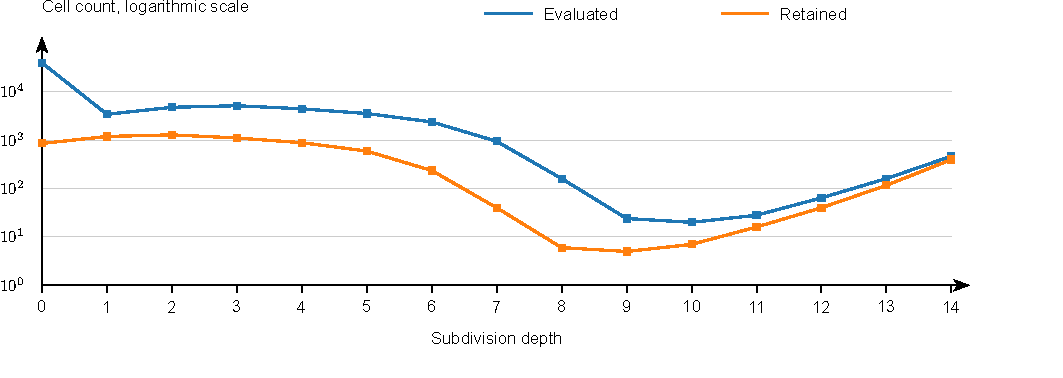
\includegraphics[width=\textwidth]{figures/pruning.pdf}
\caption{Recorded cell counts by exact subdivision depth. Retained means surviving the whole-cell predicates at that scale. Nonterminal survivors generate up to four children, so retained counts can increase while total retained area decreases. Depth 14 contains 397 terminal cells. Counts are from the saved decision replay, which matches the completed search traversal. Replay timing is excluded from the performance comparison.}
\label{fig:pruning}
\end{figure*}

\begin{figure}[t]
\centering
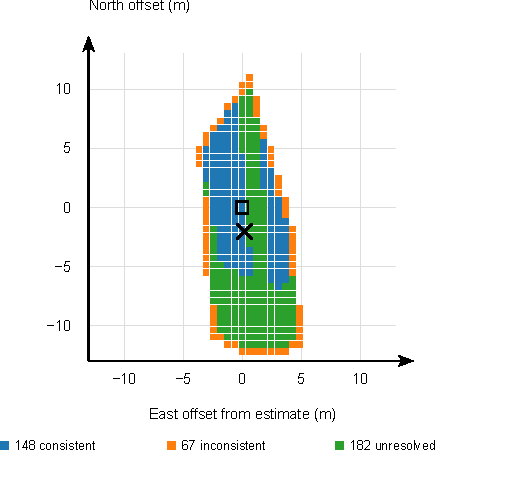
\includegraphics[width=\columnwidth]{figures/terminal.pdf}
\caption{All 397 saved terminal centers in the projected east--north frame relative to the selected estimate. The open black square marks the selected center, and the black cross marks simulated truth. Colored squares distinguish pointwise certification statuses. Surrounding terminal cells remain retained regardless of the center label.}
\label{fig:terminal}
\end{figure}

\section{Recorded Charleston Evaluation}
\subsection{Inputs, Timing, and Coverage}
The evaluated frame simulates an observer at $32.770000^\circ$ north, $79.905000^\circ$ west. It contains 70 reports, comprising 64 physical aids and six vessels. A 10 km sensor range is used. The search covers the original Eastern Seaboard rectangle, with east span 1,644.676 km and north span 2,388.459 km. It begins with a $165\times239$ array of 39,435 cells of nominal 10 km width. Edge cells can be clipped by the domain. The terminal threshold is 1 m, producing a nominal interior dyadic width of $10{,}000/2^{14}=0.61035$ m. This geometric resolution is distinct from estimation accuracy.

The chart source is the National Oceanic and Atmospheric Administration Electronic Navigational Chart (NOAA ENC) Direct GIS extract, combined with an ENC shoreline mosaic. The canonical world contains 32,168 chart objects and 2,268 vessel records, for 34,436 objects in total. Its prepared land layer contains 11,274,092 boundary segments, with separate coverage and unknown-region layers. The sensor angular resolution is $0.1^\circ$.

The search uses three NVIDIA RTX 6000 Ada Generation GPUs, each with approximately 48 GB memory, on an Intel Xeon w9-3495X host with 56 physical cores. Geometry, bearings, and assignment costs use 64-bit floating-point arithmetic. Recorded batches contain up to 512 cells, root tasks contain up to eight roots, and nearby-object capacity is 2,048 per candidate. A 2 GB per-device workspace budget bounds temporary allocation. Capacity exhaustion retains uncertainty rather than truncating possible objects.

The saved updated search completed in 8.461936 s on devices 0--2. Every root was completed exactly once across 4,930 scheduled tasks. Independent saved-output verification counted 13,899, 13,552, and 11,984 roots on the respective devices. Search time includes device setup, coordination, synchronization, and output work inside the search operation. It excludes the separate input/cache-loading phase.

The complete recorded pipeline took 23.449 s, including 7.388 s of input/cache loading, selection from saved outputs, separate truth evaluation, and cache-preservation checks. Both caches were loaded without rebuilding, and their hashes, sizes, and modification times matched before and after. Consequently, 8.462 s describes this search stage with reusable prepared inputs, while 23.449 s describes the wider recorded pipeline \cite{Vaught2026CharlestonRecord}.

\begin{table}[t]
\caption{Saved Same-Frame Search Comparison}
\label{tab:comparison}
\centering
\begin{tabular}{lrr}
\toprule
Quantity & Preceding search & Revised search\\
\midrule
Initial cells & 39,435 & 39,435\\
Evaluated regions & 1,337,411 & 64,875\\
Whole-cell rejections & 976,768 & 58,118\\
Terminal centers & 36,149 & 397\\
Consistent centers & 148 & 148\\
Unresolved centers & 15,441 & 182\\
Search time (s) & 98.495290 & 8.461936\\
\bottomrule
\end{tabular}
\end{table}

\subsection{Measured Pruning Effectiveness}
Table~\ref{tab:comparison} compares the updated search with the preceding saved full-coast search. Input hashes, settings, devices, and every-tenth-batch profiling were identical. The revised search evaluated 95.149\% fewer regions, reduced terminal centers by 98.902\%, and produced an observed search-time ratio of 11.640. The selected position, residual, and all 148 consistent terminal rectangles, flags, and assignments remained identical. This is a paired observation for one corrected frame, without repeated-run timing statistics.

The saved decision trace contains all 64,875 evaluated rectangles. Of these, 58,118 were rejected, 6,360 were expanded, and 397 became terminal. Whole-cell rejection therefore accounts for 89.585\% of evaluated decisions. At the root scale, 38,584 of 39,435 cells were rejected, or 97.842\%, leaving 851 cells for subdivision. This first stage removes large areas, while later angular contraction resolves ambiguities that cannot be excluded at 10 km scale.



The trace attributes 5,931 rejections to whole-cell land, 39,011 to a positive report with no possible object, 475 to too few possible distinct objects, and 12,701 to failure of injective assignment after the simpler tests. The last category is 21.854\% of recorded rejections. These are the reported decision categories under the executed predicate order. They are not independent causal contributions because a cell can satisfy more than one impossibility condition.

Figure~\ref{fig:pruning} shows how ambiguity changes with scale. At depths seven and eight, the survivor population falls from 40 to six cells. It later increases locally because finer rectangles tile the small still-possible region. Increasing terminal count near the solution therefore does not indicate that remote alternatives have reappeared. The saved replay took 8.681850 s with observation and recording overhead. That value is a diagnostic recording duration and is not substituted for the original 8.461936 s search measurement.

\subsection{Selected Position and Remaining Local Ambiguity}
The selected estimate is $32.7700183883^\circ$ north, $79.9050031341^\circ$ west. It matches all 64 positive reports with consistent status, zero flags, and summed absolute bearing residual $6.280980^\circ$. Truth remained separate until after the estimate was frozen. WGS84 ellipsoidal distance without fitted alignment gives a position error of 2.060304 m \cite{Vaught2026CharlestonRecord}.



The final population contains 148 consistent, 67 inconsistent, and 182 unresolved centers. All terminal centers lie within 12.717 m of the selected estimate, and all unresolved centers lie within 12.135 m. Consistent centers extend up to 8.548 m from it. These distances describe saved sampled centers, rather than confidence intervals or a continuous feasible-set radius. Figure~\ref{fig:terminal} shows their local arrangement. No remote terminal cell remains in the completed declared domain under the accepted pruning premises.

The unresolved centers require careful interpretation. Their nominal assignments match 60--63 reports and carry zero numerical flags, yet the raw-object graph still permits a complete explanation. The raw graph does not apply the full polygon sight-line test, and the saved universal rectangular barrier set is empty. Detailed nominal prediction does apply shoreline occlusion and angular grouping. Possible graph explanations can therefore remain that are occluded or incompatible with nominal grouping. The record does not establish a cause for each unresolved center.

All 15,441 formerly unresolved centers were removed by revised whole-cell pruning. However, the 182 current unresolved centers were previously labeled inconsistent by nominal grouping alone. They are retained because separating physical impossibility from nominal failure prevents unsupported rejection. This status change is a correctness distinction as well as a reduction in candidate count. The 67 inconsistent center labels must also be distinguished from the separate 67 whole-cell rejections at the final subdivision level. Equal counts do not make them the same decisions.

\section{Discussion and Conclusion}
The observed speed follows from three linked choices. First, complete-domain subdivision makes coarse impossibility proofs eliminate descendants. Second, true-bearing intervals and simultaneous distinct-object matching make those proofs selective enough to remove nearly all coarse coastal alternatives. Third, static indexing and device-resident parallel arithmetic reduce the repeated cost of evaluating the remaining cells. The recorded comparison supports their combined effect while preserving the previous consistent solution set.

The guarantees remain conditional on the model. Trusted aid detections must represent true distinct physical objects, true-north heading must be supplied, angular errors must respect the hard bound, and chart identity and position support must match the asserted catalog. Shoreline coverage and numerical bounds must support each conclusion that depends on them. Heading uncertainty, false aid detections, uncertain chart positions, or map errors require correspondingly wider support or a revised observation model. The current experiment does not characterize those cases.

The result establishes that one corrected simulated Charleston frame can be searched over the declared Eastern Seaboard domain in a recorded 8.462 s, producing a selected error of 2.060 m while preserving all unresolved local alternatives. The next technical step is a certified visibility-and-grouping test for remaining conservative graph explanations. Broader multi-site and field evidence is then needed to characterize accuracy, ambiguity, and runtime across conditions. The present record provides a concrete method and traceable reduction in completed-search work without treating a successful sampled fix as proof of unique localization.

\bibliographystyle{IEEEtran}
\bibliography{references}
\end{document}
